\documentclass{article}


\usepackage{tikz}
\usetikzlibrary{arrows}
\usepackage{amsthm, amsmath, amssymb}
\usepackage{enumitem}
\usepackage{mathtools}
\usepackage{etoolbox}
\mathtoolsset{centercolon} 
\DeclarePairedDelimiter\abs{\lvert}{\rvert}
\DeclarePairedDelimiter\ang{\langle}{\rangle}

\theoremstyle{plain}
\newtheorem{theorem}{Theorem}
\newtheorem{lemma}[theorem]{Lemma}
\theoremstyle{remark}
\newtheorem{claim}{Claim}
\theoremstyle{definition}
\newtheorem{exercise}{Exercise}



\DeclareMathOperator{\Aut}{Aut}
\DeclareMathOperator{\rot}{rot}
\def\IM{\text{Im}}
\def\inv{^{-1}}
\def\SL{\text{SL}_2(\mathbb R)}
\def\H{\mathbb{H}}
\def\D{\mathbb{D}}
\def\R{\mathbb{R}}
\def\C{\mathbb{C}}
\renewcommand{\vec}[1]{\mathbf{#1}}
\DeclarePairedDelimiterX\norm[1]\lVert\rVert{
	\ifblank{#1}{\:\cdot\:}{#1}
}



\usepackage{enumitem}
\def\labelenumi{\textbf{(\alph*)}}
\usepackage[inline]{asymptote}
\def\asydir{./asydir}




\title{Notes on Differential Geometry}
\author{\textsc{Sivmeng Hun}}
\date{\today}

\begin{document}
\maketitle

\section{Curves}

\noindent\hrulefill
\begin{exercise}
  Find a parametrized curve $\alpha(t)$ whose trace is the
  circle $x^2+y^2=1$ such that $\alpha(t)$ runs clockwise
  around the circle with $\alpha(0)=(0,1)$.
\end{exercise}
\noindent\hrulefill
\begin{proof}[Solution]
  We start with the curve $r_1(t) = (\cos t,\sin t)$, where $t\in[0,2\pi)$. 
  \begin{center}
    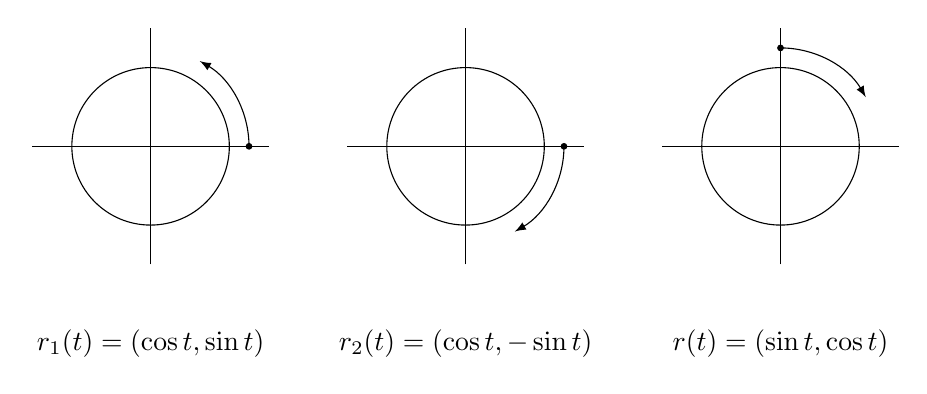
\begin{tikzpicture}
      \draw (-1.5,0)--(1.5,0) (0,-1.5)--(0,1.5);
      \draw (0,0) circle (1);
      \draw[-latex] (0:1.25) arc (0:60:1.25);
      \draw[fill=black] (0:1.25) circle (1pt);
      \node at (0,-2.5) {$r_1(t)=(\cos t, \sin t)$};

      \begin{scope}[xshift=4cm]
        \draw (-1.5,0)--(1.5,0) (0,-1.5)--(0,1.5);
        \draw (0,0) circle (1);
        \draw[-latex] (0:1.25) arc (0:-60:1.25);
        \draw[fill=black] (0:1.25) circle (1pt);
        \node at (0,-2.5) {$r_2(t)=(\cos t, -\sin t)$};
      \end{scope}

      \begin{scope}[xshift=8cm]
        \draw (-1.5,0)--(1.5,0) (0,-1.5)--(0,1.5);
        \draw (0,0) circle (1);
        \draw[-latex] (90:1.25) arc (90:30:1.25);
        \draw[fill=black] (90:1.25) circle (1pt);
        \node at (0,-2.5) {$r(t)=(\sin t,\cos t)$};
        % \node at (0,-2.5) {$r(t)=(\cos(t-\frac\pi 2), -\sin(t-\frac\pi 2))$};
      \end{scope}
    \end{tikzpicture}
  \end{center}
  By negating the sign of the second coordinate of $r_1$,  we get the curve $r_2$
  that starts at $(1,0)$ and runs clockwise.
  By replacing $t\mapsto t-\frac\pi 2$, we get the curve $r_3$ that still runs
  clockwise but whose starting point is $(0,1)$. Therefore,
  $\alpha(t)=(\sin t, \cos t)$ is the desired parametrized curve.
\end{proof}

\noindent\hrulefill
\begin{exercise}
  Let $\alpha(t)$ be a parametrized curve which does not pass through the origin.
  If $\alpha(t_0)$ is a point of the trace of $\alpha$ closest to the origin and
  $\alpha'(t_0)\neq\vec{0}$, show that the position vector $\alpha(t_0)$
  is orthogonal to $\alpha'(t_0)$.
\end{exercise}
\noindent\hrulefill
\begin{proof}
  Because $\abs{\alpha(t)}\neq 0$ for all $t$,
  the real-valued function $\abs{\alpha}$ is differentiable whose derivative is
  \begin{align*}
    \frac{d}{dt}\abs{\alpha(t)}
    &= \frac{d}{dt}\sqrt{\ang{\alpha, \alpha}}\\
    &= \frac{\ang{\alpha',\alpha}+\ang{\alpha,\alpha'}}{2\sqrt{\ang{\alpha,\alpha}}}\\
    &= \frac1{\abs{\alpha}}\cdot\ang{\alpha,\alpha'}.
  \end{align*}
  Moreover $\abs{\alpha}$ has minimun when $t=t_0$, thus the derivative of $\abs{\alpha}$
  is zero there. Hence
  \[\ang{\alpha(t_0), \alpha'(t_0)}=0,\]
  thus the two vectors are orthogonal.
  %% TODO: Need picture
\end{proof}

\noindent\hrulefill
\begin{exercise}
  A parametrized curve $\alpha(t)$ has the property that its second derivative
  $\alpha''(t)$ is identically zero. What can be said about $\alpha$?
\end{exercise}
\noindent\hrulefill
\begin{proof}[Answer]
  My guess is that $\alpha$ is a line.
\end{proof}

\noindent\hrulefill
\begin{exercise}
  Let $\alpha:I\to\R^3$ be a parametrized curve and let $v\in\R^3$ be a fixed
  vector. Assume that $\alpha'(t)$ is orthogonal to $v$ for all $t\in I$ and
  that $\alpha(0)$ is also orthogonal to $v$. Prove that $\alpha(t)$ is
  orthogonal to $v$ for all $t\in I$.
\end{exercise}
\noindent\hrulefill
\begin{proof}
  We have the following
  \[\frac{d}{dt}\ang{\alpha, v} = \ang{\alpha',v}+\ang{\alpha,v'}=0. \]
  Thus the inner product $\ang{\alpha(t), v}=c$ is a constant for all $t$.
  Since $\alpha(0)$ is also orthogonal to $v$ then $\ang{\alpha(0), v}=0$.
  We must $c=0$, which concludes the proof.
\end{proof}


\noindent\hrulefill
\begin{exercise}
  Let $\alpha:I\to\R^3$ be a parametrized curve, with $\alpha'(t)\neq 0$ for all $t\in I$.
  Show that $\abs{\alpha(t)}$ is a nonzero constant if and only if $\alpha(t)$
  is orthogonal to $\alpha'(t)$ for all $t\in I$.
\end{exercise}
\noindent\hrulefill
\begin{proof}[Answer]
  Use $\frac d{dt}\abs{\alpha}=\frac1{\alpha}\ang{\alpha,\alpha'}$, I think.
\end{proof}

\noindent\hrulefill
\begin{exercise}
  Show that the tanget lines to the regular parametrized curve
  $\alpha(t)=(3t,3t^2,2t^3)$ make a constant angle with the line $y=0, z=x$.
\end{exercise}
\noindent\hrulefill
\begin{proof}
  The tangent is $\alpha'(t)=(3,6t,6t^2)$. Because the angle of the tangent with the line
  $y=0,z=x$ is the angle between $\alpha'$ and $n=(1,0,1)$, and if $\theta$ is this
  angle we then have
  \begin{align*}
    \cos\theta
    = \frac{\ang{\alpha', n}}{\abs{\alpha'}\abs{n}}
    = \frac{3+6t^2}{\sqrt{9(1+4t^2+4t^4)}\cdot\sqrt{2}}
    = \frac1{\sqrt 2}.
  \end{align*}
  Thus at any point, the angle is always constant.
\end{proof}


\noindent\hrulefill
\begin{exercise}
  A circular disk of radius $1$ in the plane $xy$ rolls without slipping
  along the $x$ axis.
  \begin{enumerate}
  \item
    Obtain a parametrized curve $\alpha:\R\to\R^2$ the trace of which is
    the cycloid, and determine its singular points.
  \item 
    Compute the arc length of the cycloid corresponding to a complete
    rotation of the disk.
  \end{enumerate}
\end{exercise}
\noindent\hrulefill
\begin{proof}[Solution]
  \text{}
  \begin{enumerate}
  \item
    Because the cycloid the periodic in the period of $2\pi$, it's then
    enough to only parametrize $\alpha:[0,2\pi]\to \R^2$.
    \begin{center}
      \begin{asy}
import graph;
import geometry;
import settings;

outformat = "pdf";
unitsize(1.25cm);
defaultpen(fontsize(10pt));
size(10cm);

pair cycloid(real t){
	return (t-sin(t), 1-cos(t));
}

real t0=2.4;
pair A = (t0, 0);
pair C = (t0,1);
pair D = cycloid(t0);

draw(A--C--D);
draw(circle( C,1 ));
markangle( D, C, A, radius=0.2cm, L=Label("$t$") );
markangle( (D.x,0),D,C, radius=0.2cm, n=2, space=0.05cm, L=Label("$\beta$", Fill(white)) );
draw( (D.x,0)--D--(0,D.y), p=Dotted);
distance(Label("$t$"), (0,0), A, 0.8cm);

draw(graph(cycloid, 0, 2*pi+2));
draw( (-0.5,0)--(2*pi+1.5,0) );
draw( (0,-0.25)--(0,2.25) );

dot("$D$", D, N+W);
dot("$A$", (0,D.y), 1.2W);
dot("$B$", (D.x,0), 1.2S);
dot("$O$", (0,0), S+W);
dot(C);
      \end{asy}
    \end{center}
    The angle $\beta=\pi-t$, using some trigs give us:
    \begin{align*}
      &OA = 1 + \cos\beta = 1-\cos t\\
      &OB=t-\sin\beta = t-\sin t
    \end{align*}
    Therefore, we can parametrized the cycloid $\alpha:[0,2\pi]\to\R^2$ by
    \[\alpha(t)=(1-\cos t, t-\sin t).\]
    
  \item The arc length correspond to a full rotation is
    \begin{align*}
      L
      &= \int_0^{2\pi}\abs{\alpha'(u)}du\\
      &= \int_0^{2\pi}\sqrt{ (1-\cos u)^2 + \sin^2u }du\\
      &= \int_0^{2\pi}\sqrt{1-2\cos u+\cos^2u+\sin^2u}du\\
      &= \int_0^{2\pi}\sqrt{2}\cdot\sqrt{2\sin^2\frac u2}du\\
      &= \Big[ -4\cos\frac u2\Big]_0^{2\pi} = 8
    \end{align*}
  \end{enumerate}
\end{proof}










\end{document}